\chapter{System Model}
\label{cha:system}
\vspace{0.4 cm}

Write about the system model ...


\section{System architecture}
\label{sec:architecture}
\vspace{0.2 cm}

Describe the system architecture ...

\begin{figure}[ht]
\centering 
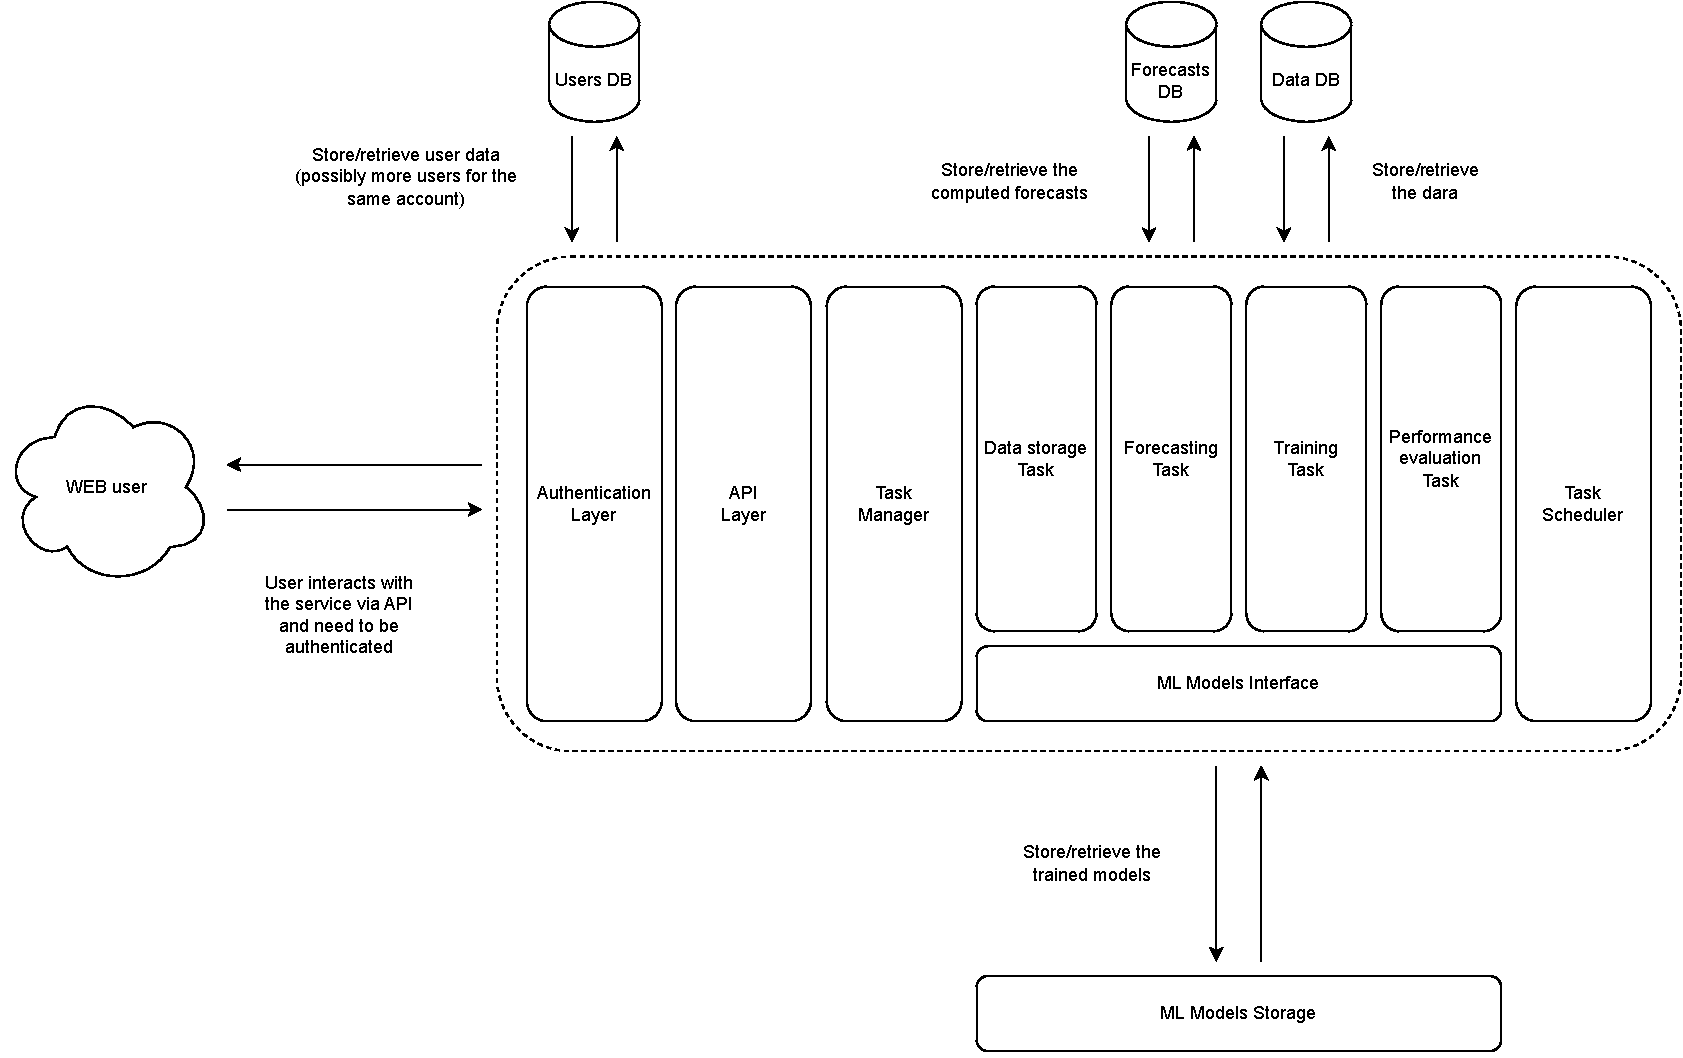
\includegraphics[width=0.9\textwidth]{images/architecture_components} 
\caption{Architecture of the proposed system.}
\label{fig:components}
\end{figure}

\begin{figure}[ht]
\centering 
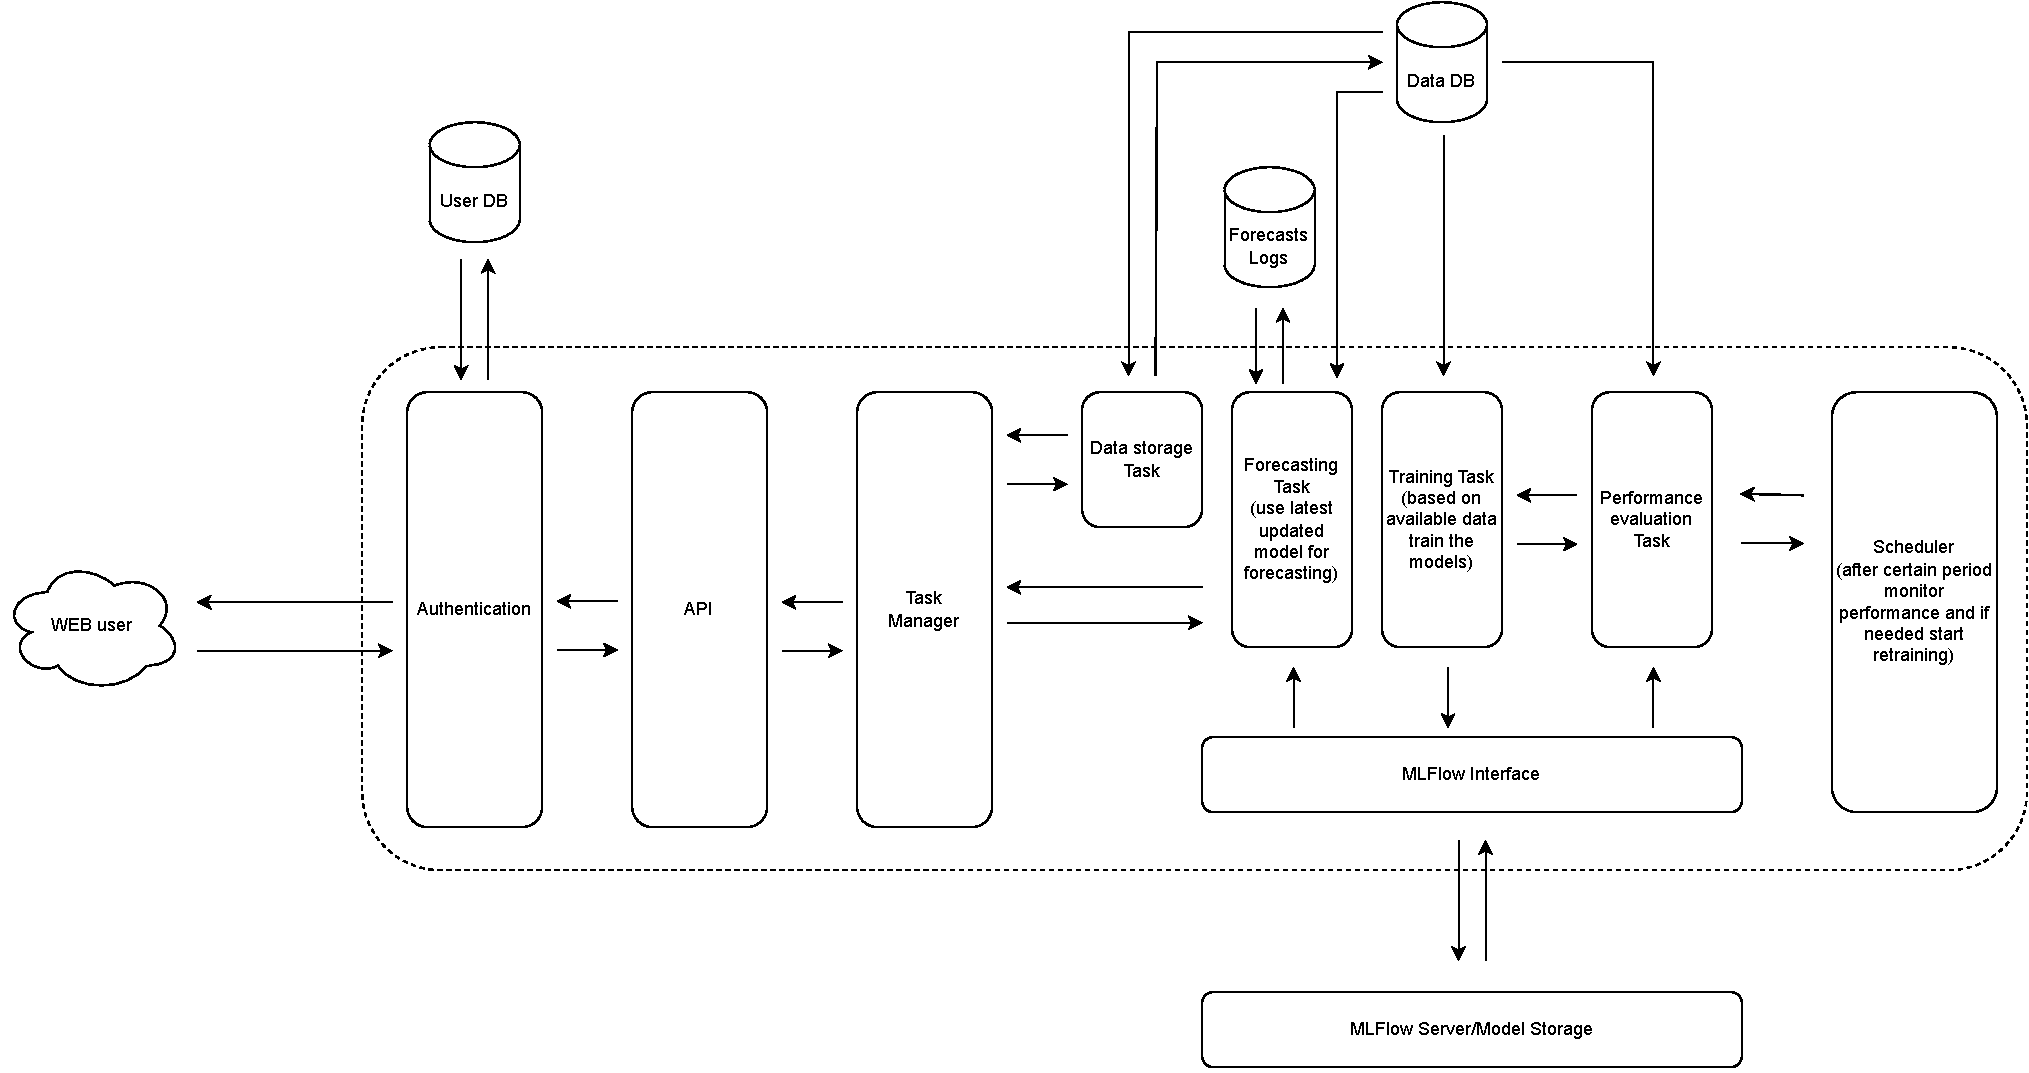
\includegraphics[width=0.9\textwidth]{images/architecture_interactions} 
\caption{Interaction of the components of the proposed system.}
\label{fig:interactions}
\end{figure}

\begin{figure}[ht]
\centering 
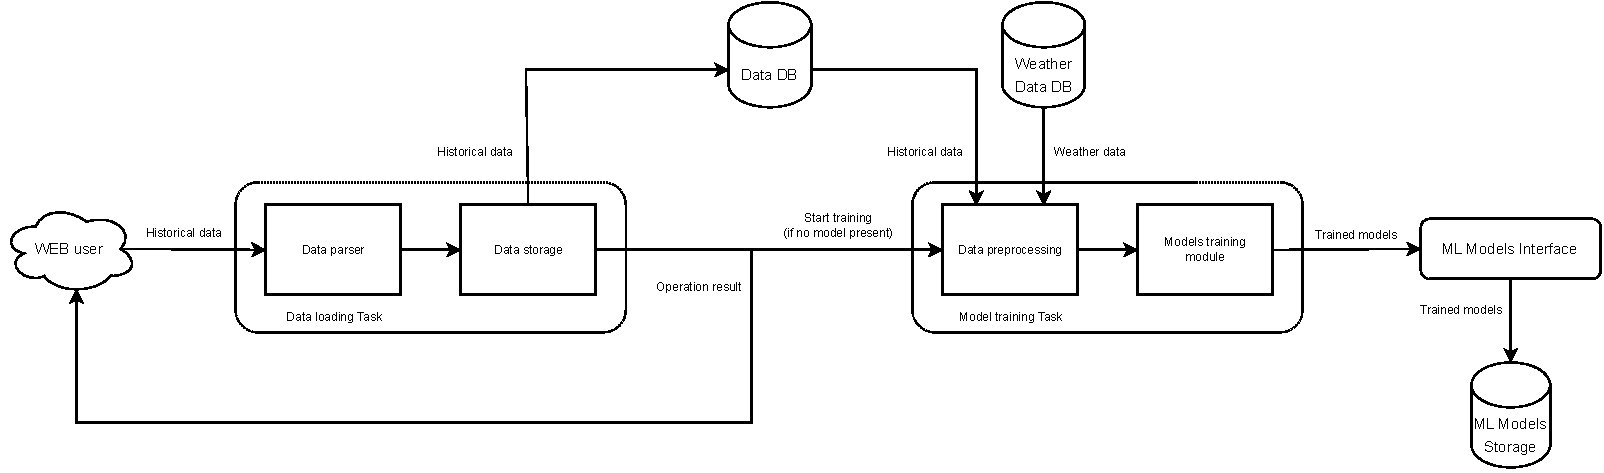
\includegraphics[width=0.9\textwidth]{images/architecture_data_loading_flow} 
\caption{Data loading flow.}
\label{fig:loadingflow}
\end{figure}

\begin{figure}[ht]
\centering 
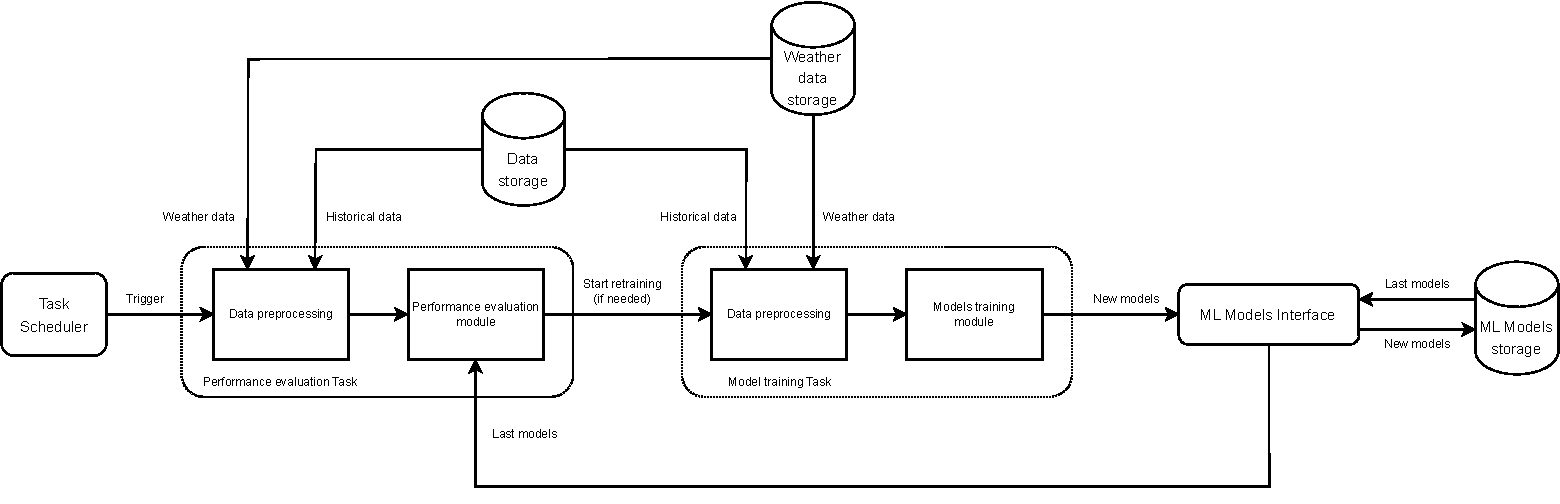
\includegraphics[width=0.9\textwidth]{images/architecture_scheduler_flow} 
\caption{Scheduler flow.}
\label{fig:schedulerflow}
\end{figure}

\begin{figure}[ht]
\centering 
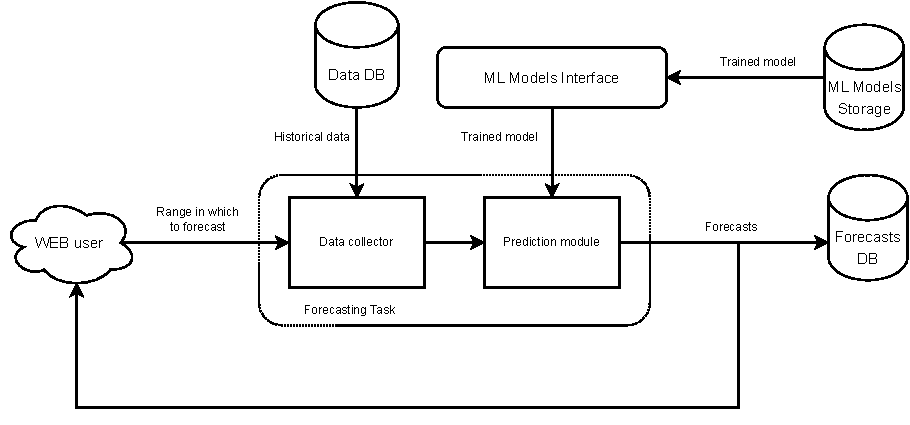
\includegraphics[width=0.9\textwidth]{images/architecture_forecast_flow} 
\caption{Forecast flow.}
\label{fig:forecastflow}
\end{figure}

\begin{figure}[ht]
\centering 
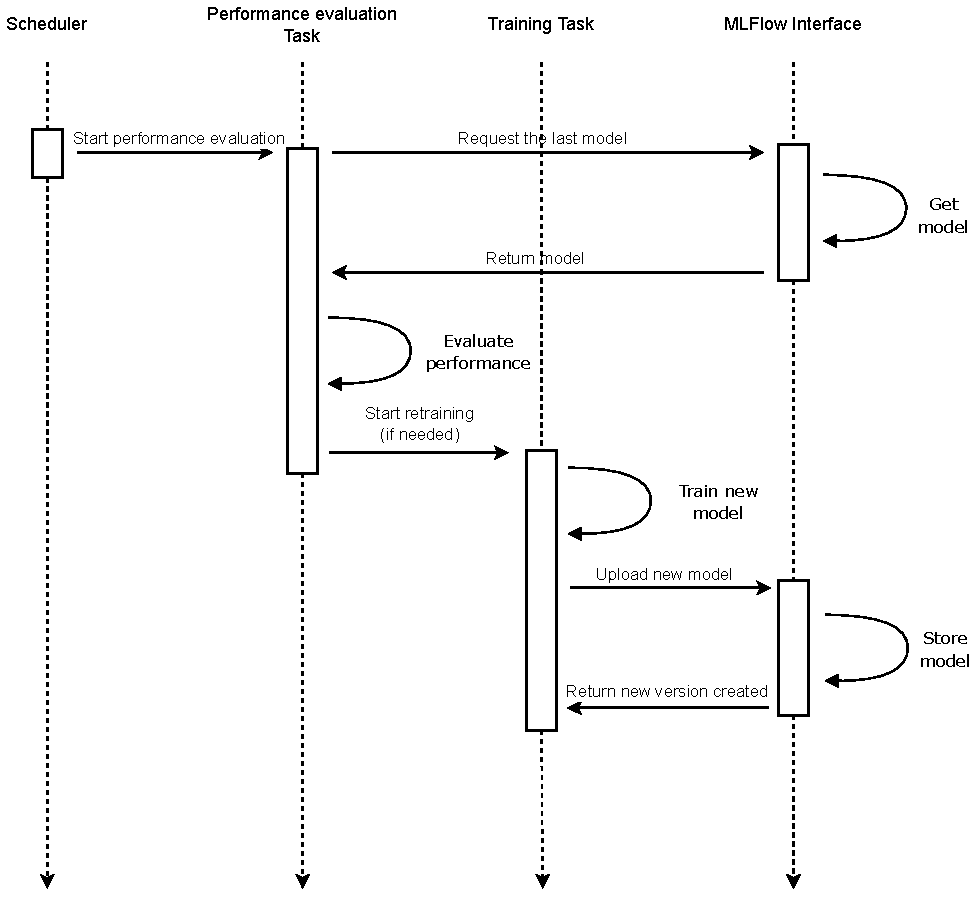
\includegraphics[width=0.9\textwidth]{images/architecture_scheduler_sequence} 
\caption{Scheduler sequence diagram.}
\label{fig:schedulersequence}
\end{figure}

\begin{figure}[ht]
\centering 
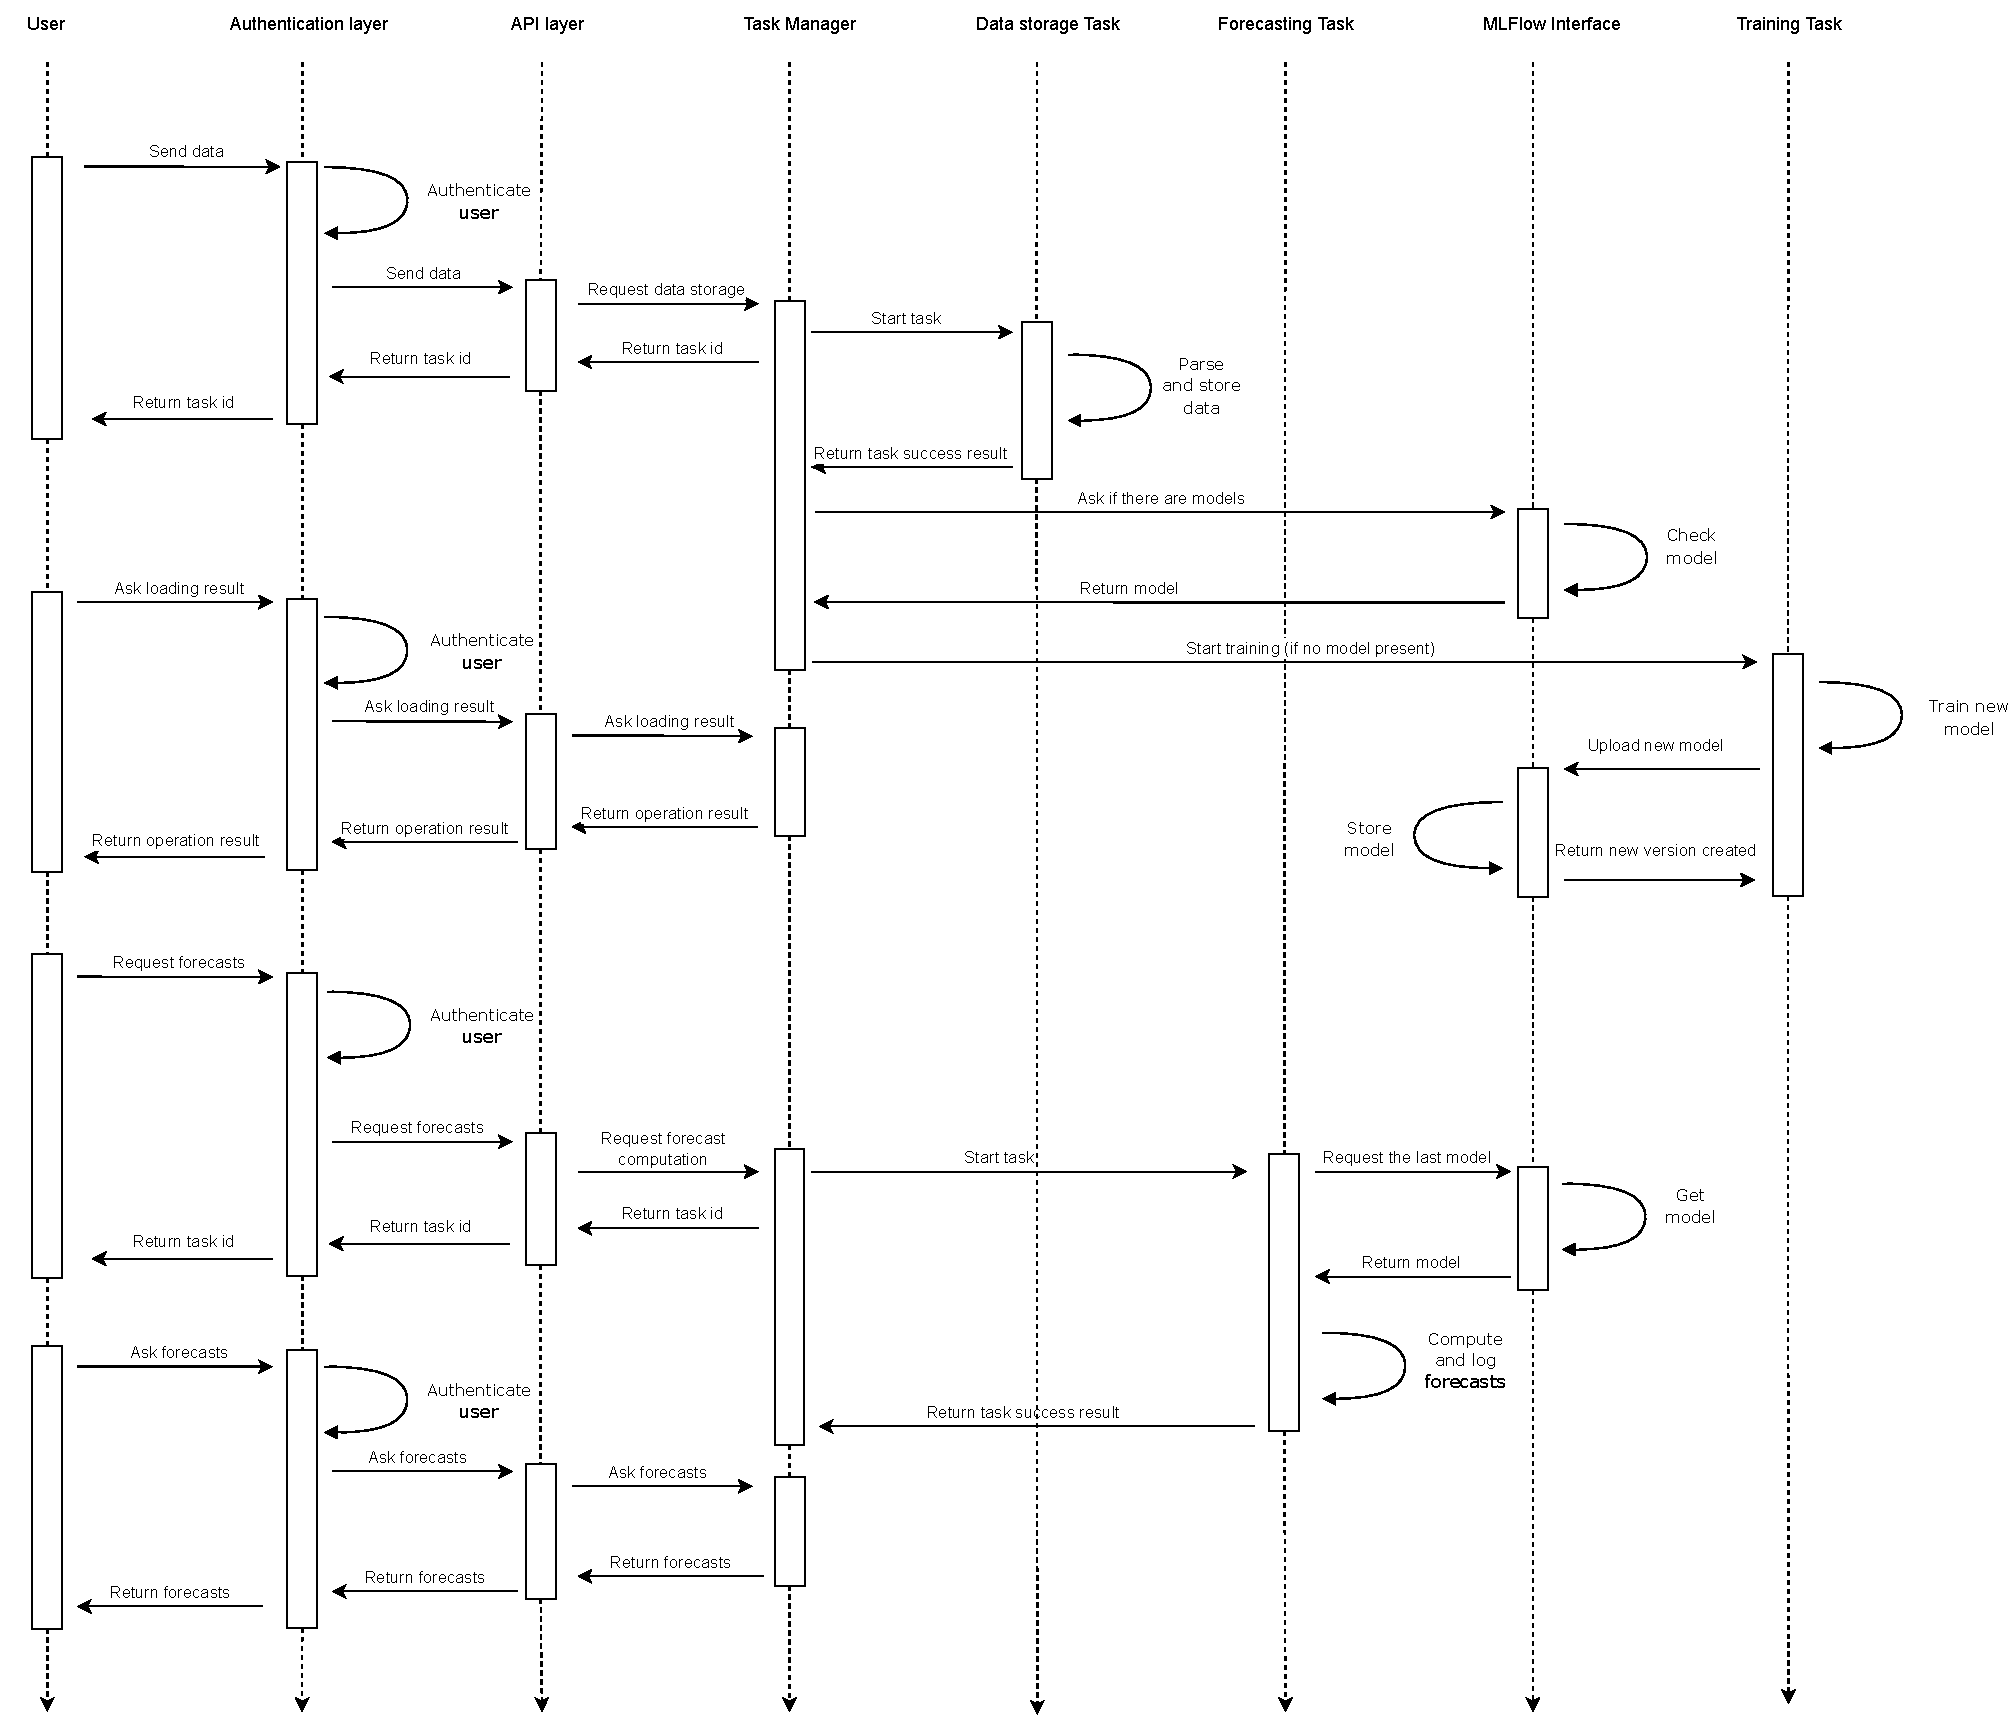
\includegraphics[width=0.9\textwidth]{images/architecture_user_sequence} 
\caption{User sequence diagram.}
\label{fig:usersequence}
\end{figure}

\begin{figure}[ht]
\centering 
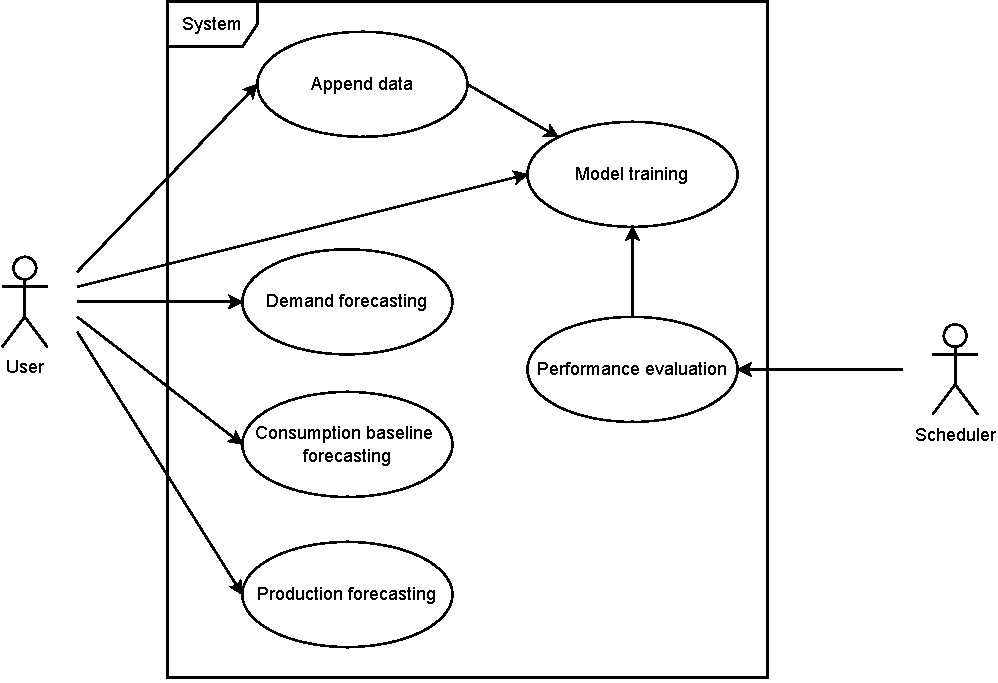
\includegraphics[width=0.9\textwidth]{images/architecture_use_case} 
\caption{Use case diagram.}
\label{fig:usecase}
\end{figure}


\section{Common components}
\label{sec:components}
\vspace{0.2 cm}

Describe the common components ...

\begin{figure}[ht]
\centering 
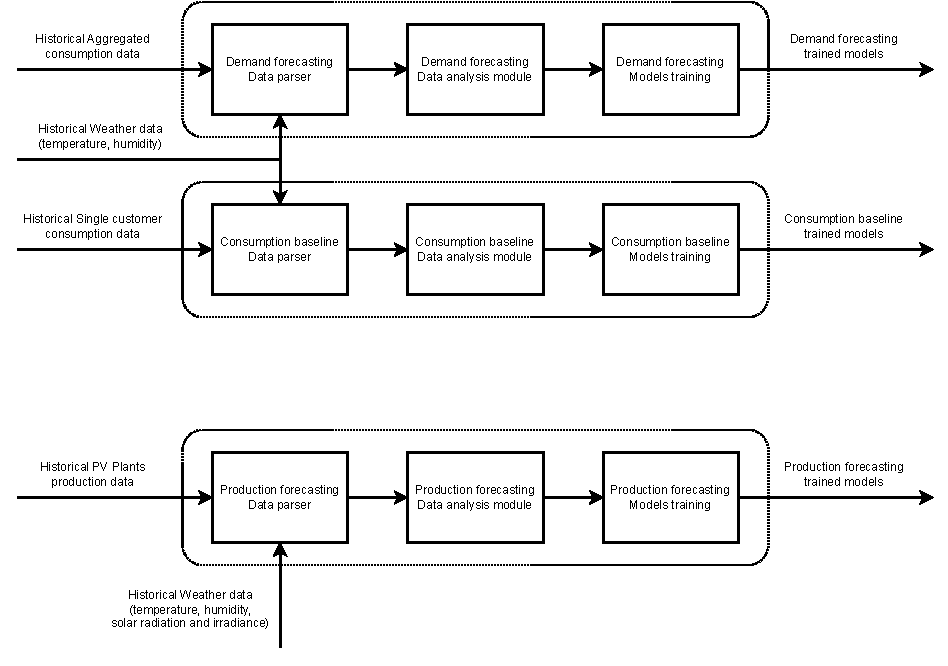
\includegraphics[width=0.9\textwidth]{images/system_model_training} 
\caption{System model training.}
\label{fig:modeltraining}
\end{figure}

\begin{figure}[ht]
\centering 
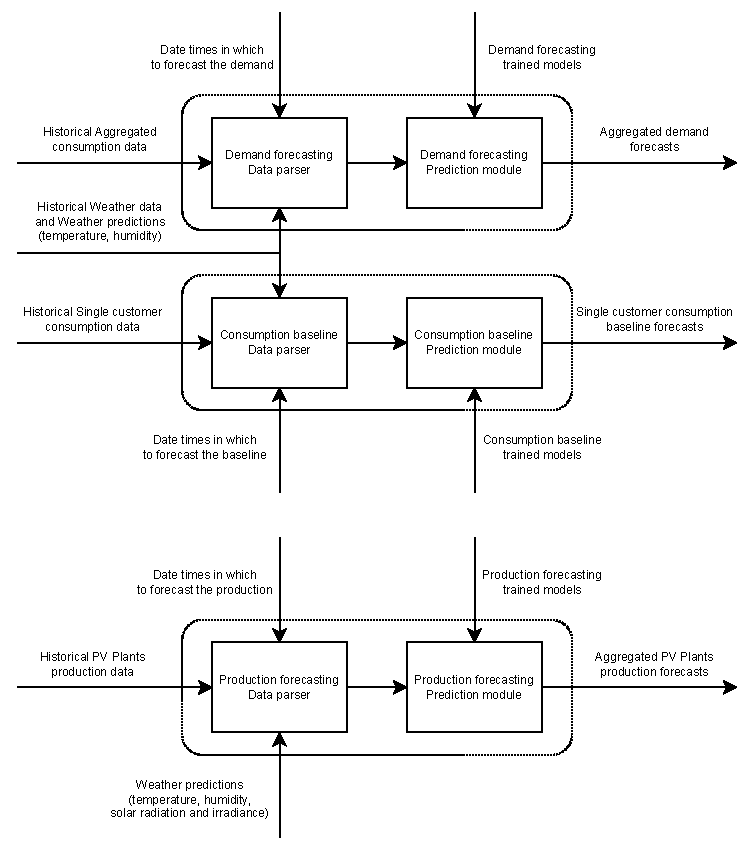
\includegraphics[width=0.9\textwidth]{images/system_model_forecasting} 
\caption{System model forecasting.}
\label{fig:modelforecasting}
\end{figure}


\section{Electricity demand forecasting}
\label{sec:demandmodel}
\vspace{0.2 cm}

Describe the electricity demand forecasting model ...


\section{Consumption baseline forecasting}
\label{sec:baselinemodel}
\vspace{0.2 cm}

Describe the consumption baseline forecasting model ...


\section{Electricity production forecasting}
\label{sec:productionmodel}
\vspace{0.2 cm}

Describe the electricity production forecasting model ...
